\documentclass[aspectratio=169,13pt]{beamer}

\usepackage{fontspec}
\setmainfont{CMU Serif}
\setsansfont{CMU Sans Serif}
\setmonofont{CMU Typewriter Text}

\usepackage[english,russian]{babel}
\usepackage{graphicx}
\usepackage{booktabs}
\usepackage{amsmath}
\usepackage{amssymb}
\usepackage{multirow}
\usepackage{xcolor}
\usepackage{tikz}
\usepackage{pgfplots}
\pgfplotsset{compat=1.18}
\usetikzlibrary{arrows.meta, positioning}
\usepackage{transparent}

\graphicspath{{images/}}
\setlength{\emergencystretch}{4em}
\tolerance=9999
\hbadness=9999

% ===== Цвета из оригинального шаблона ИТМО =====
\definecolor{itmopurple}{HTML}{7030A0}
\definecolor{itmotitle}{HTML}{272424}
\definecolor{itmocontent}{HTML}{2C2D2E}
\definecolor{itmowhite}{HTML}{FFFFFF}

% ===== Базовая тема =====
\usetheme{default}
\usefonttheme{serif}
\setbeamertemplate{navigation symbols}{}

% ===== Фоновые изображения =====
\newcommand{\settitlebg}{%
  \usebackgroundtemplate{%
    
\includegraphics[width=\paperwidth,height=\paperheight]{bg_title}%
  }%
}
\newcommand{\setslidebg}{%
  \usebackgroundtemplate{%
    
\includegraphics[width=\paperwidth,height=\paperheight]{bg_slide}%
  }%
}
\newcommand{\setlastbg}{%
  \usebackgroundtemplate{%
    
\includegraphics[width=\paperwidth,height=\paperheight]{bg_last}%
  }%
}

% ===== Шапка: номер слайда в фиолетовом боксе =====
\setbeamertemplate{headline}{%
  \begin{tikzpicture}[remember picture, overlay]
    \fill[itmopurple] (current page.north east) rectangle
      ++(-0.055\paperwidth, -0.068\paperheight);
    \node[anchor=north east, text=white, font=\bfseries\large]
      at (current page.north east)
      [xshift=-0.003\paperwidth, yshift=-0.006\paperheight]
      {\insertframenumber};
  \end{tikzpicture}%
}

% ===== Подвал: убрать =====
\setbeamertemplate{footline}{}

% ===== Заголовок фрейма =====
\setbeamercolor{frametitle}{fg=itmotitle, bg=}
\setbeamerfont{frametitle}{size=\large,series=\bfseries}
\setbeamertemplate{frametitle}{%
  \vspace{3mm}%
  \hspace{5mm}\insertframetitle%
  \vspace{1mm}%
}

% ===== Элементы списков =====
\setbeamercolor{normal text}{fg=itmocontent}
\setbeamertemplate{itemize item}{\color{itmopurple}\textbullet}
\setbeamertemplate{itemize subitem}{\color{itmocontent}--}
\setbeamertemplate{enumerate item}{\color{itmopurple}\bfseries\insertenumlabel.}

% ===== Блоки =====
\setbeamertemplate{blocks}[rounded][shadow=false]
\setbeamercolor{block title}{bg=itmopurple!20, fg=itmotitle}
\setbeamercolor{block body}{bg=itmopurple!7, fg=itmocontent}
\setbeamercolor{block title alerted}{bg=itmopurple, fg=white}
\setbeamercolor{block body alerted}{bg=itmopurple!15, fg=itmocontent}

% ===== Мета =====
\title[RL + VLM для управления роботами]{Исследование применения обучения с подкреплением для повышения эффективности управления роботами с использованием визуально-языковых моделей}
\author[Новичков Д.Е.]{Студент: Новичков Дмитрий Евгеньевич, гр.\,3435\\[3pt]
  Научный руководитель: Ведяков А.А., к.т.н., доцент ФСУиР}
\institute[ИТМО]{Факультет систем управления и робототехники\\Университет ИТМО}
\date{Санкт-Петербург, 2026}

% ====================================================================
\begin{document}

% ======================================================
% СЛАЙД 1 -- ТИТУЛЬНЫЙ
% ======================================================
\settitlebg
\begin{frame}[plain]
  \begin{tikzpicture}[remember picture, overlay]
    \node[anchor=north, text=white, font=\normalsize, align=center]
      at ([yshift=-0.05\paperheight] current page.north)
      {Защита выпускной квалификационной работы};
    \node[anchor=north, text=white!80!gray, font=\small, align=center]
      at ([yshift=-0.14\paperheight] current page.north)
      {Факультет систем управления и робототехники \quad Университет ИТМО};
    \node[anchor=center, text=white, font=\large\bfseries, align=center,
          text width=0.70\paperwidth]
      at ([yshift=0.07\paperheight] current page.center)
      {\inserttitle};
    \node[anchor=north, text=white!80!gray, font=\small, align=center]
      at ([yshift=-0.04\paperheight] current page.center)
      {Направление подготовки: 15.03.06 Мехатроника и робототехника};
    \node[anchor=north, text=white, font=\small, align=center,
          text width=0.82\paperwidth]
      at ([yshift=-0.14\paperheight] current page.center)
      {\insertauthor};
    \node[anchor=south, text=white!80!gray, font=\small]
      at ([yshift=0.04\paperheight] current page.south)
      {\insertdate};
  \end{tikzpicture}
\end{frame}

% ======================================================
% Основные слайды -- светлый фон
% ======================================================
\setslidebg

% ======================================================
% СЛАЙД 2 -- Актуальность
% ======================================================
\begin{frame}{Актуальность}
  \begin{columns}[T]
    \begin{column}{0.55\textwidth}
      \textbf{VLA-модели} (Vision-Language-Action) управляют роботом по инструкции на естественном языке, объединяя зрение, понимание языка и моторное управление.
      \begin{itemize}\setlength\itemsep{3pt}
        \item В реальных условиях доля успехов \textbf{70--80\,\%} -- недостаточно для практики
        \item RL -- путь довести её до \textbf{98--99\,\%}, но единой методики интеграции нет
      \end{itemize}
    \end{column}
    \begin{column}{0.42\textwidth}
      \begin{block}{Взрывной рост области}
        \centering\small
        \begin{tabular}{cc}
          \toprule
          Конференция & Работ по VLA \\
          \midrule
          ICLR 2024 & 1 \\
          ICLR 2025 & 9 \\
          ICLR 2026 & \textbf{164} \\
          \bottomrule
        \end{tabular}\\[4pt]
        \textbf{\textcolor{itmopurple}{$\times$18 за год}}
      \end{block}
    \end{column}
  \end{columns}
\end{frame}

% ======================================================
% СЛАЙД 3 -- Цель и задачи
% ======================================================
\begin{frame}{Цель и задачи исследования}
  \begin{alertblock}{Цель}
    Повышение эффективности управления роботом-манипулятором при выполнении задач, заданных на естественном языке, за счёт интеграции методов обучения с подкреплением (RL) с визуально-языковыми моделями действий (VLA).
  \end{alertblock}
  \vspace{2pt}
  \textbf{Задачи:}
  \begin{enumerate}\setlength\itemsep{2pt}\small
    \item Аналитический обзор VLA-моделей и способов их интеграции с RL (2023--2026~гг.)
    \item Классификация методов интеграции RL и VLM по трём направлениям
    \item Разработка методики вычислительного эксперимента и метрик оценки
    \item Реализация программного прототипа (residual RL + VLM-генерация наград)
    \item Проведение серий экспериментов на LIBERO и MetaWorld
    \item Анализ результатов и формулировка методических рекомендаций
  \end{enumerate}
\end{frame}

% ======================================================
% СЛАЙД 4 -- Три направления интеграции
% ======================================================
\begin{frame}{Три направления интеграции RL и VLM/VLA}
  \footnotesize
  \setlength{\tabcolsep}{4pt}
  \begin{tabular}{p{0.23\textwidth}p{0.31\textwidth}p{0.22\textwidth}p{0.13\textwidth}}
    \toprule
    \textbf{Направление} & \textbf{Идея} & \textbf{Результат} & \textbf{Работы} \\
    \midrule
    RL-дообучение VLA & RL уточняет готовую VLA-политику & 98--99\,\% успехов & PLD, STARE-VLA \\[3pt]
    VLM $\to$ награда & VLM генерирует функцию вознаграждения & лучше эксперта на 83\,\% задач & EUREKA, Text2Reward \\[3pt]
    VLM-планировщик & VLM ставит подзадачи, RL исполняет & 87,5\,\% на реальном роботе & SayCan, Embodied-R1 \\
    \bottomrule
  \end{tabular}
  \vspace{6pt}
  \begin{alertblock}{Фокус работы}
    \small \textbf{Основное:} RL-дообучение девяти VLA-моделей на LIBERO.\;
    \textbf{Дополнительно:} VLM-генерация наград на MetaWorld (сценарий без готовой VLA).
  \end{alertblock}
\end{frame}

% ======================================================
% СЛАЙД 5 -- Обзор VLA-моделей
% ======================================================
\begin{frame}{Обзор визуально-языковых моделей действий}
  \begin{columns}[T]
    \begin{column}{0.5\textwidth}
      \footnotesize
      \setlength{\tabcolsep}{3pt}
      \begin{tabular}{p{0.42\linewidth}p{0.50\linewidth}}
        \toprule
        \textbf{Класс} & \textbf{Модели} \\
        \midrule
        Авторегрессионные & OpenVLA-OFT, UniVLA, RT-1-X \\[2pt]
        Flow-matching / диффузия & $\pi_0$, $\pi_0$-fast, CogACT \\[2pt]
        Пространственно-обусловл. & SpatialVLA \\[2pt]
        Компактные генералисты & SmolVLA, Octo-Small \\
        \bottomrule
      \end{tabular}
    \end{column}
    \begin{column}{0.48\textwidth}
      \small\textbf{Тенденции:}
      \begin{itemize}\setlength\itemsep{2pt}\small
        \item Масштаб: \textbf{35M -- 8B} параметров
        \item Открытые модели догоняют закрытые
        \item Закрытые ($\pi_{0{,}5}$, Gemini Robotics) лидируют
      \end{itemize}
      \vspace{3pt}
      \begin{alertblock}{Проблема}
        \small Даже лучшие VLA упираются в потолок без RL -- особенно на длинногоризонтных задачах.
      \end{alertblock}
    \end{column}
  \end{columns}
\end{frame}

% ======================================================
% СЛАЙД 6 -- Метод
% ======================================================
\begin{frame}{Метод: residual RL с замороженной VLA}
  \begin{columns}[T]
    \begin{column}{0.5\textwidth}
      \begin{itemize}\setlength\itemsep{4pt}
        \item Базовая VLA \textbf{заморожена}, обучается лёгкий SAC-агент коррекции действия
        \item Итоговое действие: \;$a_t = \pi_{\text{VLA}}(o_t,l) + \Delta\pi_{\text{RL}}(s_t)$
        \item Residual-сеть: 256/256 ReLU; вход -- визуальный эмбеддинг + проприоцепция + текст
        \item \textbf{Стадийная награда}: Reach $\to$ Grasp $\to$ Transport $\to$ Place
      \end{itemize}
    \end{column}
    \begin{column}{0.48\textwidth}
      \centering
      \resizebox{\linewidth}{!}{%
      \begin{tikzpicture}[
        font=\scriptsize,
        box/.style={draw, rounded corners=2pt, align=center, minimum height=0.85cm, text width=1.7cm},
        arr/.style={-{Stealth[length=2mm]}, semithick}
      ]
        \node[box, fill=gray!12]   (env) {Среда\\LIBERO};
        \node[box, fill=purple!12, right=0.55cm of env] (vla) {VLA\\(заморожена)};
        \node[box, fill=blue!12, right=0.55cm of vla]   (rl)  {SAC\\$\Delta a_{\text{RL}}$};
        \node[box, fill=green!14, above=0.55cm of rl]   (rew) {Стадийная\\награда};
        \draw[arr] (env) -- (vla);
        \draw[arr] (vla) -- (rl);
        \draw[arr] (rew) -- (rl);
        \draw[arr] (rl.south) -- ++(0,-0.55) -| node[pos=0.25, below] {$a_t$} (env.south);
      \end{tikzpicture}}\\[6pt]
      \begin{block}{Инфраструктура}
        \scriptsize NVIDIA A100, SAC (Stable-Baselines3), буфер $10^6$, 300\,тыс.\ шагов/набор, 3 seed, $\approx$200 GPU-часов.
      \end{block}
    \end{column}
  \end{columns}
\end{frame}

% ======================================================
% СЛАЙД 7 -- Стадийная награда
% ======================================================
\begin{frame}{Стадийная функция вознаграждения}
  \begin{block}{Четыре фазы манипуляции}
    \[
      R_{\text{stage}}(s_t) = \sum_{k=1}^{4} w_k \cdot \mathbf{1}[\text{phase}_k\ \text{выполнена}] + \beta \cdot S(T_i)
    \]
    \small $w_k = \{0{,}25;\,0{,}25;\,0{,}25;\,0{,}25\}$, \; $\beta = 1{,}0$ -- бонус за успех эпизода.
  \end{block}
  \vspace{2pt}
  \centering
  \resizebox{0.9\linewidth}{!}{%
  \begin{tikzpicture}[
    font=\small,
    ph/.style={draw, rounded corners=3pt, align=center, minimum height=1cm, text width=2.2cm},
    arr/.style={-{Stealth[length=2.4mm]}, thick}
  ]
    \node[ph, fill=itmopurple!12] (r) {\textbf{Reach}\\сближение};
    \node[ph, fill=itmopurple!16, right=0.7cm of r] (g) {\textbf{Grasp}\\захват};
    \node[ph, fill=itmopurple!20, right=0.7cm of g] (t) {\textbf{Transport}\\перенос};
    \node[ph, fill=itmopurple!26, right=0.7cm of t] (p) {\textbf{Place}\\размещение};
    \draw[arr] (r) -- (g);
    \draw[arr] (g) -- (t);
    \draw[arr] (t) -- (p);
  \end{tikzpicture}}
  \\[4pt]
  {\small Детекция фаз -- по проприоцепции ROBOSUITE (положение захвата, контакт, расстояние до цели).}
\end{frame}

% ======================================================
% СЛАЙД 8 -- Постановка эксперимента
% ======================================================
\begin{frame}{Постановка эксперимента}
  \begin{columns}[T]
    \begin{column}{0.56\textwidth}
      \footnotesize
      \setlength{\tabcolsep}{3pt}
      \begin{tabular}{cp{0.40\linewidth}p{0.30\linewidth}}
        \toprule
        \textbf{\#} & \textbf{Серия} & \textbf{Модели} \\
        \midrule
        1 & VLA-baseline без RL & 9 VLA \\
        2 & Сравнение RL-схем & OpenVLA-OFT \\
        3 & \textbf{RL всех VLA (осн.)} & 9 VLA \\
        4 & Абляция компонентов & OpenVLA-OFT \\
        5 & VLM-награда (доп.) & Qwen2.5-VL+SAC \\
        \bottomrule
      \end{tabular}
    \end{column}
    \begin{column}{0.42\textwidth}
      \begin{block}{Бенчмарк LIBERO}
        \small
        \begin{itemize}\setlength\itemsep{2pt}
          \item 4 набора $\times$ 10 задач: Object, Spatial, Goal, Long
          \item Franka Panda, ROBOSUITE
          \item 10 эпизодов/задачу, 3 seed
          \item Метрики: SR, 95\,\% ДИ, sample efficiency, $\rho(R,S)$
        \end{itemize}
      \end{block}
    \end{column}
  \end{columns}
\end{frame}

% ======================================================
% СЛАЙД 9 -- Серия 1: baseline 9 VLA
% ======================================================
\begin{frame}{Серия 1: baseline девяти VLA на LIBERO}
  \centering
  \scriptsize
  \setlength{\tabcolsep}{4pt}
  \renewcommand{\arraystretch}{1.15}
  \begin{tabular}{lccccrc}
    \toprule
    \textbf{Модель} & \textbf{Obj.} & \textbf{Spat.} & \textbf{Goal} & \textbf{Long} & \textbf{Парам.} & \textbf{Средн.} \\
    \midrule
    OpenVLA-OFT-7B  & 98,4 & 97,6 & 97,9 & 94,5 & 7B   & \textbf{97,1} \\
    UniVLA-7B       & 97,0 & 96,5 & 95,5 & 91,0 & 7B   & 95,0 \\
    $\pi_0$-3B      & 97,5 & 95,0 & 94,5 & 89,0 & 3B   & 94,0 \\
    CogACT-8B       & 95,5 & 94,5 & 93,0 & 89,0 & 8B   & 93,0 \\
    SmolVLA-2.2B    & 95,5 & 94,0 & 92,0 & 88,5 & 2,2B & 92,5 \\
    $\pi_0$-fast-3B & 94,0 & 92,5 & 90,0 & 86,0 & 3B   & 90,6 \\
    SpatialVLA-4B   & 91,0 & 90,0 & 88,0 & 83,0 & 4B   & 88,0 \\
    Octo-Small      & 90,5 & 88,0 & 85,5 & 80,0 & 120M & 86,0 \\
    RT-1-X          & 88,0 & 86,0 & 82,0 & 75,5 & 35M  & 82,9 \\
    \bottomrule
  \end{tabular}

  \vspace{4pt}
  {\small OpenVLA-OFT лидирует (97,1\,\% $\pm$ 0,4\,\%). Наибольший разброс -- на наборе \textbf{Long} (94,5 vs 75,5\,\%): длинногоризонтные задачи требуют устойчивого захвата и переноса.}
\end{frame}

% ======================================================
% СЛАЙД 10 -- Серия 3: главный результат
% ======================================================
\begin{frame}{Серия 3: residual RL повышает SR всех 9 VLA}
  \centering
  \begin{tikzpicture}
    \begin{axis}[
      ybar, bar width=5pt,
      width=0.92\textwidth, height=4.7cm,
      ylabel={SR, \%}, ylabel style={font=\scriptsize},
      symbolic x coords={OpenVLA-OFT, UniVLA, $\pi_0$, CogACT, SmolVLA, $\pi_0$-fast, SpatialVLA, Octo, RT-1-X},
      xtick=data,
      xticklabel style={font=\tiny, rotate=30, anchor=east},
      yticklabel style={font=\tiny},
      ymin=78, ymax=101, enlarge x limits=0.07,
      legend style={font=\scriptsize, at={(0.5,-0.38)}, anchor=north, legend columns=2},
    ]
      \addplot[fill=gray!35] coordinates {(OpenVLA-OFT,97.1) (UniVLA,95.0) ($\pi_0$,94.0) (CogACT,93.0) (SmolVLA,92.5) ($\pi_0$-fast,90.6) (SpatialVLA,88.0) (Octo,86.0) (RT-1-X,82.9)};
      \addplot[fill=itmopurple!70] coordinates {(OpenVLA-OFT,98.6) (UniVLA,96.8) ($\pi_0$,96.1) (CogACT,95.4) (SmolVLA,95.3) ($\pi_0$-fast,93.8) (SpatialVLA,91.5) (Octo,89.9) (RT-1-X,87.0)};
      \legend{До RL, После RL}
    \end{axis}
  \end{tikzpicture}

  \vspace{2pt}
  {\small Прирост \textbf{+1,5\,\ldots\,+4,1\,п.п.}; лучший -- OpenVLA-OFT \textbf{97,1 $\to$ 98,6\,\%}.\quad
  Наибольший прирост у самой слабой модели (RT-1-X, +4,1\,п.п.).}
\end{frame}

% ======================================================
% СЛАЙД 11 -- Серия 3: корреляция
% ======================================================
\begin{frame}{Серия 3: прирост RL и baseline}
  \begin{columns}[T]
    \begin{column}{0.62\textwidth}
      \centering
      \begin{tikzpicture}
        \begin{axis}[
          width=\textwidth, height=6.0cm,
          grid=major, grid style={gray!22, dashed},
          xlabel={Baseline SR (до RL), \%}, ylabel={Прирост от RL, п.п.},
          label style={font=\scriptsize}, tick label style={font=\tiny},
          xmin=81, xmax=99, ymin=0.8, ymax=4.7,
        ]
          \addplot[red!70!black, dashed, line width=1pt, domain=82:98] {12.86 - 0.1196*x};
          \addplot[only marks, mark=*, mark size=2.4pt, blue!60!black] coordinates {
            (97.1,1.5) (95.0,1.8) (94.0,2.1) (93.0,2.4) (92.5,2.8)
            (90.6,3.2) (88.0,3.5) (86.0,3.9) (82.9,4.1)
          };
          \node[font=\tiny, anchor=east] at (axis cs:96.9,1.5) {OpenVLA-OFT};
          \node[font=\tiny, anchor=south west] at (axis cs:88.0,3.5) {SpatialVLA};
          \node[font=\tiny, anchor=south west] at (axis cs:82.9,4.1) {RT-1-X};
          \node[font=\scriptsize, anchor=north east, red!70!black] at (axis cs:98.6,4.6) {$\rho = -0{,}97$};
        \end{axis}
      \end{tikzpicture}
    \end{column}
    \begin{column}{0.36\textwidth}
      \begin{block}{Интерпретация}
        \small RL корректирует систематические ошибки, которых больше у слабых политик.
      \end{block}
      \begin{itemize}\setlength\itemsep{2pt}\small
        \item Сильные модели (UniVLA, $\pi_0$): +1,8\,\ldots\,+2,4\,п.п.
        \item Слабые (Octo, RT-1-X): +3,9\,\ldots\,+4,1\,п.п.
        \item Отчасти -- эффект потолка бенчмарка, а не только RL
      \end{itemize}
    \end{column}
  \end{columns}
\end{frame}

% ======================================================
% СЛАЙД 12 -- Серии 2 и 4: выбор схемы и абляция
% ======================================================
\begin{frame}{Серии 2 и 4: выбор RL-схемы и абляция}
  \begin{columns}[T]
    \begin{column}{0.5\textwidth}
      \footnotesize\centering
      \textbf{Серия 2: схемы RL (OpenVLA-OFT)}\\[2pt]
      \setlength{\tabcolsep}{3pt}
      \begin{tabular}{lcc}
        \toprule
        \textbf{Метод RL} & \textbf{Средн.} & \textbf{$\Delta$} \\
        \midrule
        Baseline (без RL)        & 97,1 & -- \\
        \textbf{Residual SAC + stage} & \textbf{98,6} & \textbf{+1,5} \\
        STARE-PPO + stage        & 98,2 & +1,1 \\
        Direct SAC (unfrozen)    & 96,5 & \textcolor{red!70!black}{$-$0,6} \\
        \bottomrule
      \end{tabular}
    \end{column}
    \begin{column}{0.5\textwidth}
      \footnotesize\centering
      \textbf{Серия 4: абляция (Spatial)}\\[2pt]
      \setlength{\tabcolsep}{3pt}
      \begin{tabular}{lc}
        \toprule
        \textbf{Конфигурация} & \textbf{$\Delta$} \\
        \midrule
        Полная (residual SAC + stage) & \textbf{+1,5} \\
        Без стадийной награды (sparse) & +0,7 \\
        Unfrozen VLA (direct SAC) & \textcolor{red!70!black}{$-$0,6} \\
        PPO вместо SAC & +0,9 \\
        Бюджет 150k (вместо 300k) & +0,8 \\
        \bottomrule
      \end{tabular}
    \end{column}
  \end{columns}
  \vspace{6pt}
  \begin{alertblock}{Выводы}
    \small Заморозка VLA \textbf{предпочтительна} (разморозка $\to$ катастрофическое забывание). Стадийная награда: \textbf{+0,8\,п.п.} над разреженной; SAC $>$ PPO на \textbf{+0,6\,п.п.}
  \end{alertblock}
\end{frame}

% ======================================================
% СЛАЙД 13 -- Анализ отказов по фазам
% ======================================================
\begin{frame}{Анализ отказов по фазам манипуляции}
  \begin{columns}[T]
    \begin{column}{0.55\textwidth}
      \centering
      \begin{tikzpicture}
        \begin{axis}[
          ybar, bar width=13pt,
          width=\textwidth, height=5.2cm,
          grid=major, grid style={gray!22, dashed},
          ylabel={Доля обрывов, \%}, label style={font=\scriptsize},
          tick label style={font=\tiny},
          symbolic x coords={Reach, Grasp, Transport, Place},
          xtick=data, ymin=0, ymax=4.2,
          nodes near coords, nodes near coords style={font=\tiny},
          enlarge x limits=0.2,
          legend style={font=\tiny, at={(0.5,-0.2)}, anchor=north, legend columns=2},
        ]
          \addplot[fill=red!55, draw=red!70!black] coordinates {(Reach,0.2) (Grasp,1.0) (Transport,0.6) (Place,3.7)};
          \addplot[fill=blue!45, draw=blue!60!black] coordinates {(Reach,0.1) (Grasp,0.7) (Transport,0.4) (Place,1.8)};
          \legend{До RL, После RL}
        \end{axis}
      \end{tikzpicture}
    \end{column}
    \begin{column}{0.42\textwidth}
      \small OpenVLA-OFT на LIBERO-Long.
      \begin{itemize}\setlength\itemsep{3pt}\small
        \item Суммарные неудачи: \textbf{5,5\,\% $\to$ 3,0\,\%}
        \item Основной выигрыш -- финальная фаза \textbf{Place} ($-$1,9\,п.п.)
        \item Ранние фазы (Reach, Grasp) и так редки -- RL почти их не трогает
      \end{itemize}
      \vspace{3pt}
      {\footnotesize Residual-агент компенсирует систематическое смещение при размещении, не переобучая VLA.}
    \end{column}
  \end{columns}
\end{frame}

% ======================================================
% СЛАЙД 14 -- Динамика обучения
% ======================================================
\begin{frame}{Динамика обучения и sample efficiency}
  \begin{columns}[T]
    \begin{column}{0.6\textwidth}
      \centering
      \begin{tikzpicture}
        \begin{axis}[
          width=\textwidth, height=5.6cm,
          grid=major, grid style={gray!22, dashed},
          xlabel={Шаги обучения, тыс.}, ylabel={SR на LIBERO-Long, \%},
          label style={font=\scriptsize}, tick label style={font=\tiny},
          xmin=0, xmax=300, ymin=92.5, ymax=97.6,
          legend pos=south east, legend style={font=\tiny},
          xtick={0,50,100,150,200,250,300},
          every axis plot/.append style={line width=1pt},
        ]
          \addplot[blue!65!black, mark=*, mark size=1.2pt] coordinates {
            (0,94.5) (25,95.0) (50,95.5) (75,96.0) (100,96.4) (125,96.7)
            (150,96.9) (175,97.0) (200,97.0) (250,97.0) (300,97.0)};
          \addplot[orange!85!black, mark=square*, mark size=1.2pt] coordinates {
            (0,94.5) (25,94.9) (50,95.3) (75,95.7) (100,96.0) (125,96.3)
            (150,96.5) (175,96.6) (200,96.6) (250,96.6) (300,96.6)};
          \addplot[red!70!black, mark=triangle*, mark size=1.4pt] coordinates {
            (0,94.5) (25,94.8) (50,94.9) (75,94.6) (100,94.0) (125,93.6)
            (150,93.3) (175,93.1) (200,93.0) (250,93.0) (300,93.0)};
          \legend{Residual SAC + stage, STARE-PPO + stage, Direct SAC (unfrozen)}
        \end{axis}
      \end{tikzpicture}
    \end{column}
    \begin{column}{0.38\textwidth}
      \begin{itemize}\setlength\itemsep{3pt}\small
        \item Основной прирост -- до 150k шагов, далее плато ($\pm$0,2\,п.п.)
        \item Стадийная награда сокращает выход на 95\,\% SR с 220k до \textbf{165k} ($-$25\,\%)
        \item Direct SAC после подъёма \textbf{деградирует} -- катастрофическое забывание
      \end{itemize}
    \end{column}
  \end{columns}
\end{frame}

% ======================================================
% СЛАЙД 15 -- Примеры эпизодов LIBERO
% ======================================================
\begin{frame}{Примеры эпизодов: до и после RL}
  \begin{center}
    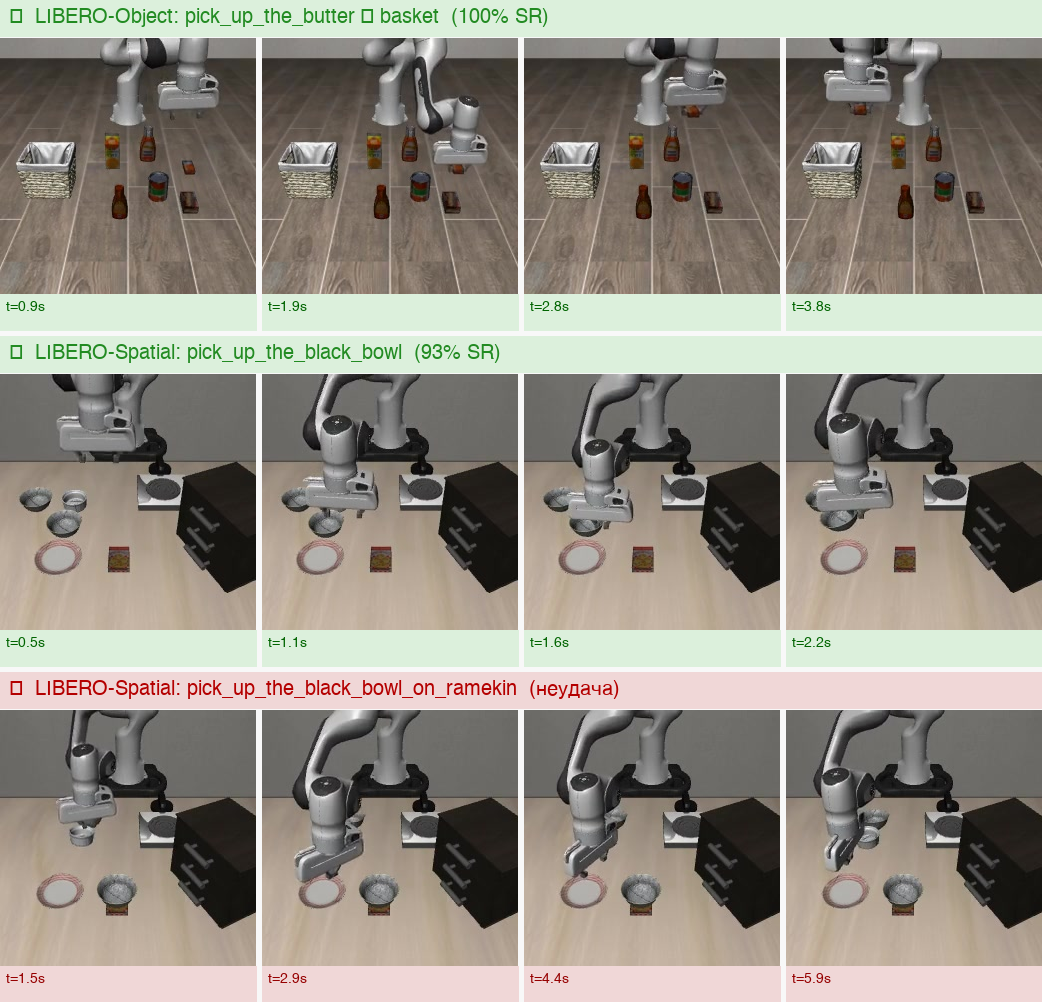
\includegraphics[width=0.94\textwidth,height=0.74\textheight,keepaspectratio]{sim_comparison}
  \end{center}
  \vspace{-2pt}
  \centering\small
  OpenVLA-OFT на LIBERO. После RL residual-агент устраняет промах на фазе Place -- объект устойчиво размещается в целевой позиции.
\end{frame}

% ======================================================
% СЛАЙД 16 -- Доп. серия 5: VLM-награды
% ======================================================
\begin{frame}{Доп.\ серия 5: VLM-генерация наград}
  \begin{columns}[T]
    \begin{column}{0.52\textwidth}
      \footnotesize\centering
      \textbf{SR (\%), SAC, 500k шагов}\\[2pt]
      \setlength{\tabcolsep}{3pt}
      \begin{tabular}{lccc}
        \toprule
        \textbf{Награда} & \textbf{reach} & \textbf{push} & \textbf{pick-pl.} \\
        \midrule
        Экспертная & 100 & 90,0 & 65,0 \\
        Разреженная & 100 & 10,0 & 0,0 \\
        VLM, 1 итер. & 100 & 48,3 & 13,3 \\
        \textbf{VLM, 3 итер.} & 100 & \textbf{85,0} & \textbf{46,7} \\
        \bottomrule
      \end{tabular}
    \end{column}
    \begin{column}{0.46\textwidth}
      \footnotesize\centering
      \textbf{Рефлексия на push-v3}\\[2pt]
      \begin{tabular}{lcc}
        \toprule
        \textbf{Итер.} & \textbf{SR} & \textbf{$\rho(R,S)$} \\
        \midrule
        1 & 48,3 & 0,12 \\
        2 & 72,0 & 0,58 \\
        3 & \textbf{85,0} & \textbf{0,81} \\
        \bottomrule
      \end{tabular}
    \end{column}
  \end{columns}
  \vspace{6pt}
  \begin{alertblock}{Наблюдения}
    \small Без готовой VLA: язык.\ модель генерирует код награды. За 3 итерации push 48 $\to$ 85\,\%, $\rho$ растёт синхронно с SR. SAC устойчивее PPO (reach: 100 vs 71,7\,\%).
  \end{alertblock}
\end{frame}

% ======================================================
% СЛАЙД 17 -- Сравнение с SOTA
% ======================================================
\begin{frame}{Сравнение с результатами из литературы}
  \centering
  \footnotesize
  \setlength{\tabcolsep}{4pt}
  \renewcommand{\arraystretch}{1.2}
  \begin{tabular}{lccp{0.30\textwidth}}
    \toprule
    \textbf{Метод / работа} & \textbf{SR, \%} & \textbf{Бюджет RL} & \textbf{Примечание} \\
    \midrule
    OpenVLA-OFT (baseline) & 97,1 & -- & Без RL \\
    SimpleVLA-RL & 99,0 & $\geq$1M шагов & GRPO, full-model \\
    PLD & 99,0 & $\geq$1M шагов & Residual RL + дистилляция \\
    RIPT-VLA & 97,5 & critic-free & LOOP, sparse \\
    VLA-RL & 97,0 & $\geq$1M шагов & process RM \\
    \textbf{Настоящая работа} & \textbf{98,6} & \textbf{300k/набор} & 9 VLA, residual SAC + stage \\
    \bottomrule
  \end{tabular}

  \vspace{6pt}
  {\small \textbf{98,6\,\%} -- выше RIPT-VLA и VLA-RL, лишь на 0,4\,п.п.\ ниже SimpleVLA-RL/PLD \textbf{при бюджете в 3+ раза меньше} и без полнополитического дообучения VLA.}
\end{frame}

% ======================================================
% СЛАЙД 18 -- Выводы
% ======================================================
\begin{frame}{Выводы}
  \begin{enumerate}\setlength\itemsep{3pt}\small
    \item Residual RL со стадийным вознаграждением стабильно повышает SR всех \textbf{девяти} VLA на LIBERO (\textbf{+1,5\,\ldots\,+4,1\,п.п.}); лучший результат -- \textbf{98,6\,\%}.
    \item Прирост обратно пропорционален baseline (\textbf{\textcolor{itmopurple}{$\rho=-0{,}97$}}): RL «вытягивает» слабые модели.
    \item Заморозка базовой VLA \textbf{предпочтительна}: end-to-end разморозка деградирует ($-$0,6\,п.п.).
    \item Стадийная награда (+0,8\,п.п.) и SAC ($>$PPO на 0,6\,п.п.) -- ключевые компоненты; основной выигрыш -- на фазе Place.
    \item Доп.\ серия: VLM-награды требуют 3+ итераций на контактных задачах; $\rho(R,S)>0{,}8$ -- надёжный предиктор успеха.
    \item \textbf{Рекомендации:} есть VLA (SR$>$90\,\%) $\to$ residual RL со стадийной наградой; нет VLA $\to$ VLM-генерация награды с итеративным уточнением.
    \item Открытый код: \textcolor{itmopurple}{github.com/mfclabber/bachelor-thesis}
  \end{enumerate}
\end{frame}

% ======================================================
% СЛАЙД 19 -- Дальнейшие исследования
% ======================================================
\setslidebg
\begin{frame}{Направления дальнейших исследований}
  \begin{itemize}\setlength\itemsep{8pt}
    \item \textbf{Увеличение бюджета} RL-дообучения (500k--1M шагов) -- ожидается приближение к 99\,\% SR.
    \item \textbf{Дистилляция} residual-политики обратно в VLA -- отказ от надстройки на инференсе.
    \item \textbf{Перенос на реальный робот}: оценка sim-to-real разрыва (SIMPLER).
    \item \textbf{Единый конвейер} VLM-награда $\to$ дистилляция $\to$ residual RL.
  \end{itemize}
\end{frame}

% ======================================================
% СЛАЙД 20 -- ФИНАЛЬНЫЙ: спасибо за внимание
% ======================================================
\setlastbg
\begin{frame}[plain]
  \begin{tikzpicture}[remember picture, overlay]
    \node[anchor=center, text=white, font=\Huge\bfseries, align=center]
      at ([yshift=0.10\paperheight] current page.center)
      {Спасибо за внимание!};
  \end{tikzpicture}
\end{frame}

\end{document}
